\section{An onset actor checkpoint repairs native recovery cost}\label{sec:p14solid}
\paragraph{Fixed design and causal contrast.} We chose one previously supported setting rather than screen additional games or report the best endpoint. Asterix PPO received reward sign corruption during updates 390--440 (409{,}600 environment steps), followed by 200 unrestricted updates. Thirty-two entirely unused training seeds 1200--1231 were fixed before target data; none of the earlier eight Asterix seeds enters this primary. The donor actor comes from the shared onset at 390, not the clean fork at 440, so it cannot import the clean agent's additional progress. All primary swaps use the exact natural damaged future context. Within pause-cell codes, C denotes the onset donor P, not extra clean-fork progress; D denotes impaired removal state. CDD therefore changes only actor parameters, whereas DCC transfers the impaired actor into onset critic/moments. The all-D cell is asserted identical over the full runner-state tree to untouched D; the unbroken clean trace supplies the historical pause benchmark. Recovery AUC excludes removal and averages the 20 checkpoints at +10--200; the late endpoint averages +160--200. No low-competence seed is filtered. Matching concerns the removal-time world/RNG/counter and initial non-actor learner fields; subsequent actions, data, critic and moments may diverge and are part of the total downstream intervention effect.

\paragraph{One registered compound result.} The single compound criterion is met, with $p_{\rm claim}=3.32\times10^{-8}$ at $\alpha=.01$; every component is reported in Table~\ref{tab:p14solid}. Native AUC cost is $-1.72\ci{-1.94}{-1.50}$, late-window cost $-1.19\ci{-1.44}{-0.93}$, and replacing only the onset actor changes AUC by $+1.58\ci{+1.37}{+1.79}$. The reciprocal actor transfer is $-1.64\ci{-1.83}{-1.45}$. Seedwise consistency is 32/32 native-negative and 32/32 rescue-positive. The repaired fraction is 91.8\% (paired-bootstrap 95\% interval 86.3--97.5\%) by ratio of paired means, not an allocation of encoded information.

\begin{table}[t]
\centering
\caption{Independent Asterix actor-repair confirmation, 32 training seeds. All four prespecified practical-effect components must pass through their maximum one-sided $p$ at $\alpha=.01$, plus at least 24/32 native-negative and rescue-positive seeds. Intervals pair independent training seeds conditional on the fixed primary evaluation batch, not episodes/checkpoints. Secondary checks cannot rescue a failed primary.}
\label{tab:p14solid}
\small
\resizebox{\linewidth}{!}{%
\begin{tabular}{lcccc}
\toprule
component & 95\% CI & 99\% CI & required mean & shifted $p$ \\
\midrule
native AUC cost & $-1.72\ci{-1.94}{-1.50}$ & $-1.72\ci{-2.02}{-1.43}$ & $<-0.50$ & $6.02\times10^{-13}$ \\
late-window cost & $-1.19\ci{-1.44}{-0.93}$ & $-1.19\ci{-1.53}{-0.84}$ & $<-0.30$ & $3.32\times10^{-8}$ \\
onset-actor rescue & $+1.58\ci{+1.37}{+1.79}$ & $+1.58\ci{+1.30}{+1.86}$ & $>+0.50$ & $4.79\times10^{-12}$ \\
reciprocal actor transfer & $-1.64\ci{-1.83}{-1.45}$ & $-1.64\ci{-1.89}{-1.38}$ & $<-0.50$ & $1.39\times10^{-13}$ \\
\bottomrule
\end{tabular}}
\end{table}
\begin{figure}[t]
\centering
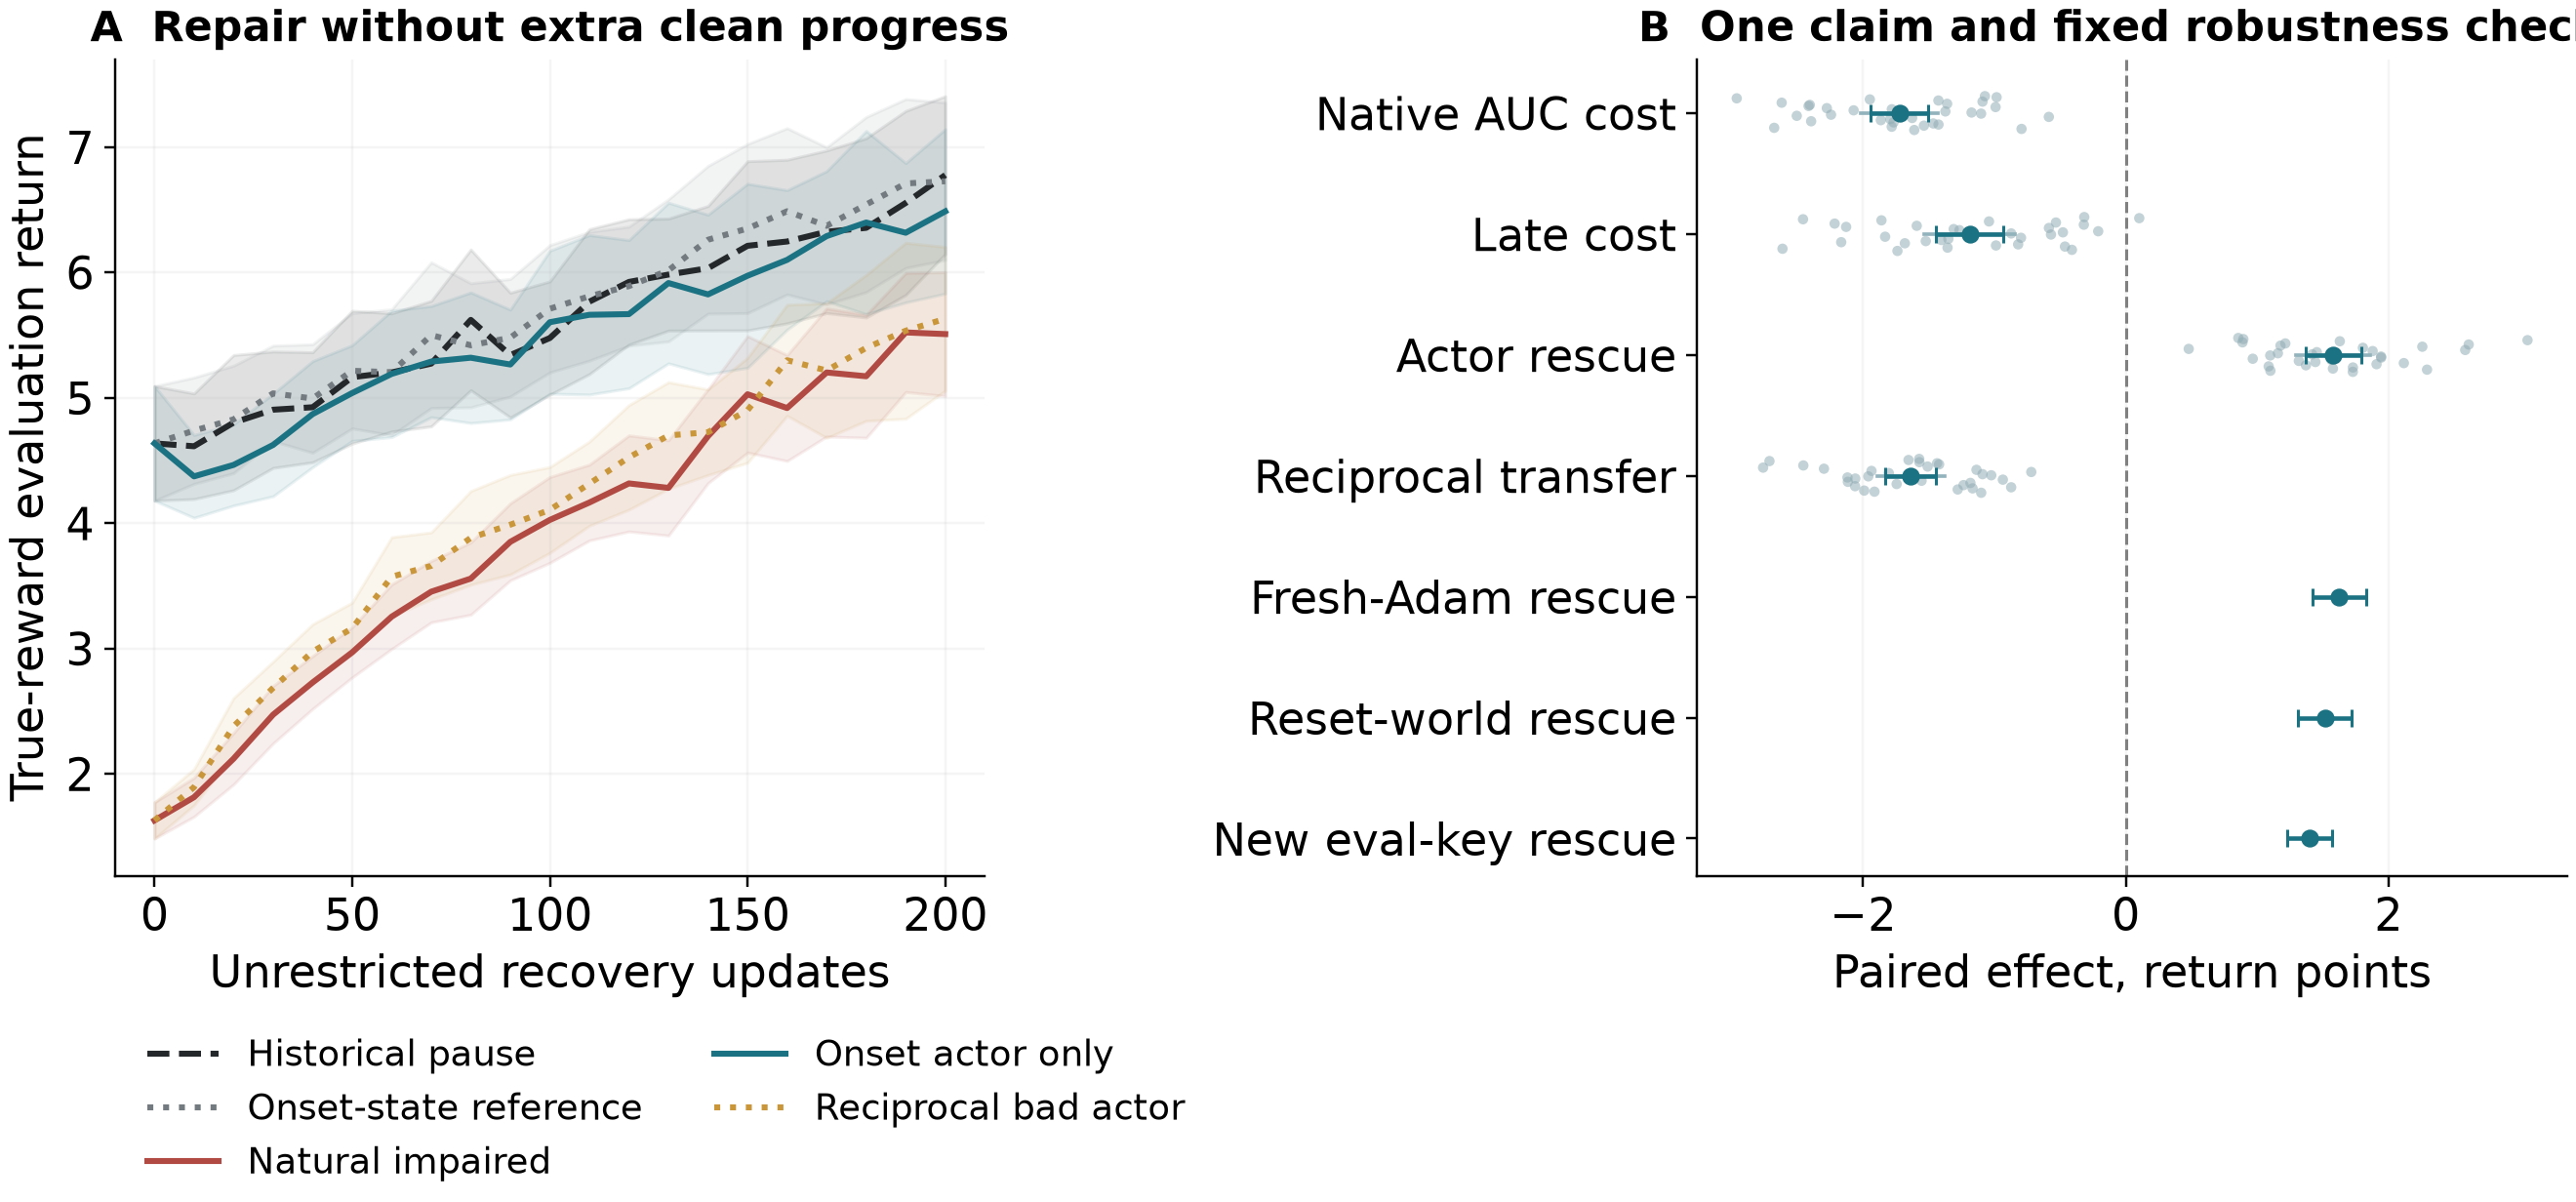
\includegraphics[width=\linewidth]{figures/p14_actor_repair.png}
\caption{One prespecified actor-repair result. At removal, the impaired and actor-repaired learners have identical natural D world/RNG/counter, critic and moments; only actor parameters change. Both then learn unrestrictedly, so downstream experience and learner fields can diverge. The reciprocal contrast is against the matched onset-state reference (CCC), not an assumed-identical historical pause. Historical pause is the earlier unbroken clean trajectory. Panel A bands are nominal pointwise 99\% seed intervals. Panel B shows 95\% intervals and, for primary components, thin 99\% whiskers. Small points in the four primary rows are all 32 paired seed effects, not selected examples. Secondary robustness is not a new primary success.}
\label{fig:p14solid}
\end{figure}

\paragraph{Prespecified robustness.} The common-fresh-Adam actor effect is $-1.59\ci{-1.77}{-1.42}$, with rescue $+1.63\ci{+1.42}{+1.83}$; reset-world rescue is $+1.52\ci{+1.31}{+1.72}$. The corresponding fresh-Adam critic effect is $-0.13\ci{-0.23}{-0.03}$, so a smaller critic effect is not declared absent. The primary conditions on the registered 64-episode evaluation batch; the second key is neither selected nor pooled into it. With independent evaluation key 54321, native cost is $-1.60\ci{-1.76}{-1.44}$, late cost $-1.07\ci{-1.31}{-0.83}$ and actor rescue $+1.40\ci{+1.23}{+1.57}$. 

\paragraph{Most of the cost, not full restoration.} Residual rescue-minus-matched-pause is $-0.23\ci{-0.37}{-0.09}$ (TOST $\pm.30$, $p=0.1599$); versus historical pause it is $-0.14\ci{-0.25}{-0.04}$ ($p=0.0021$). Matched state-pause minus historical pause is $+0.09\ci{-0.03}{+0.21}$ (TOST $\pm.30$, $p=0.0008$). The secondary historical-reference restoration margin is met, whereas the matched-state-reference margin is not met. A practical margin is not literal equality, and no full-restoration claim is made. Bootstrap, exact sign and simultaneous-bound sensitivities are in the analysis artifact. The result remains an intervention-specific, finite-horizon actor-state repair in one game and impairment family, not a unique representation mechanism, universal actor dominance or irreversible loss.
